\subsection{Thiết kế cơ sở dữ liệu}

Trong kiến trúc microservice, mỗi dịch vụ quản lý một cơ sở dữ liệu độc lập theo đúng ranh giới domain. Vì vậy, mô hình dữ liệu không sử dụng quá nhiều ràng buộc khóa ngoại như kiến trúc nguyên khối. Thay vào đó, các quan hệ giữa dữ liệu được thể hiện ở mức logic hoặc thông qua các cơ chế đồng bộ sự kiện giữa các dịch vụ.

\begin{figure}[H]
    \centering
    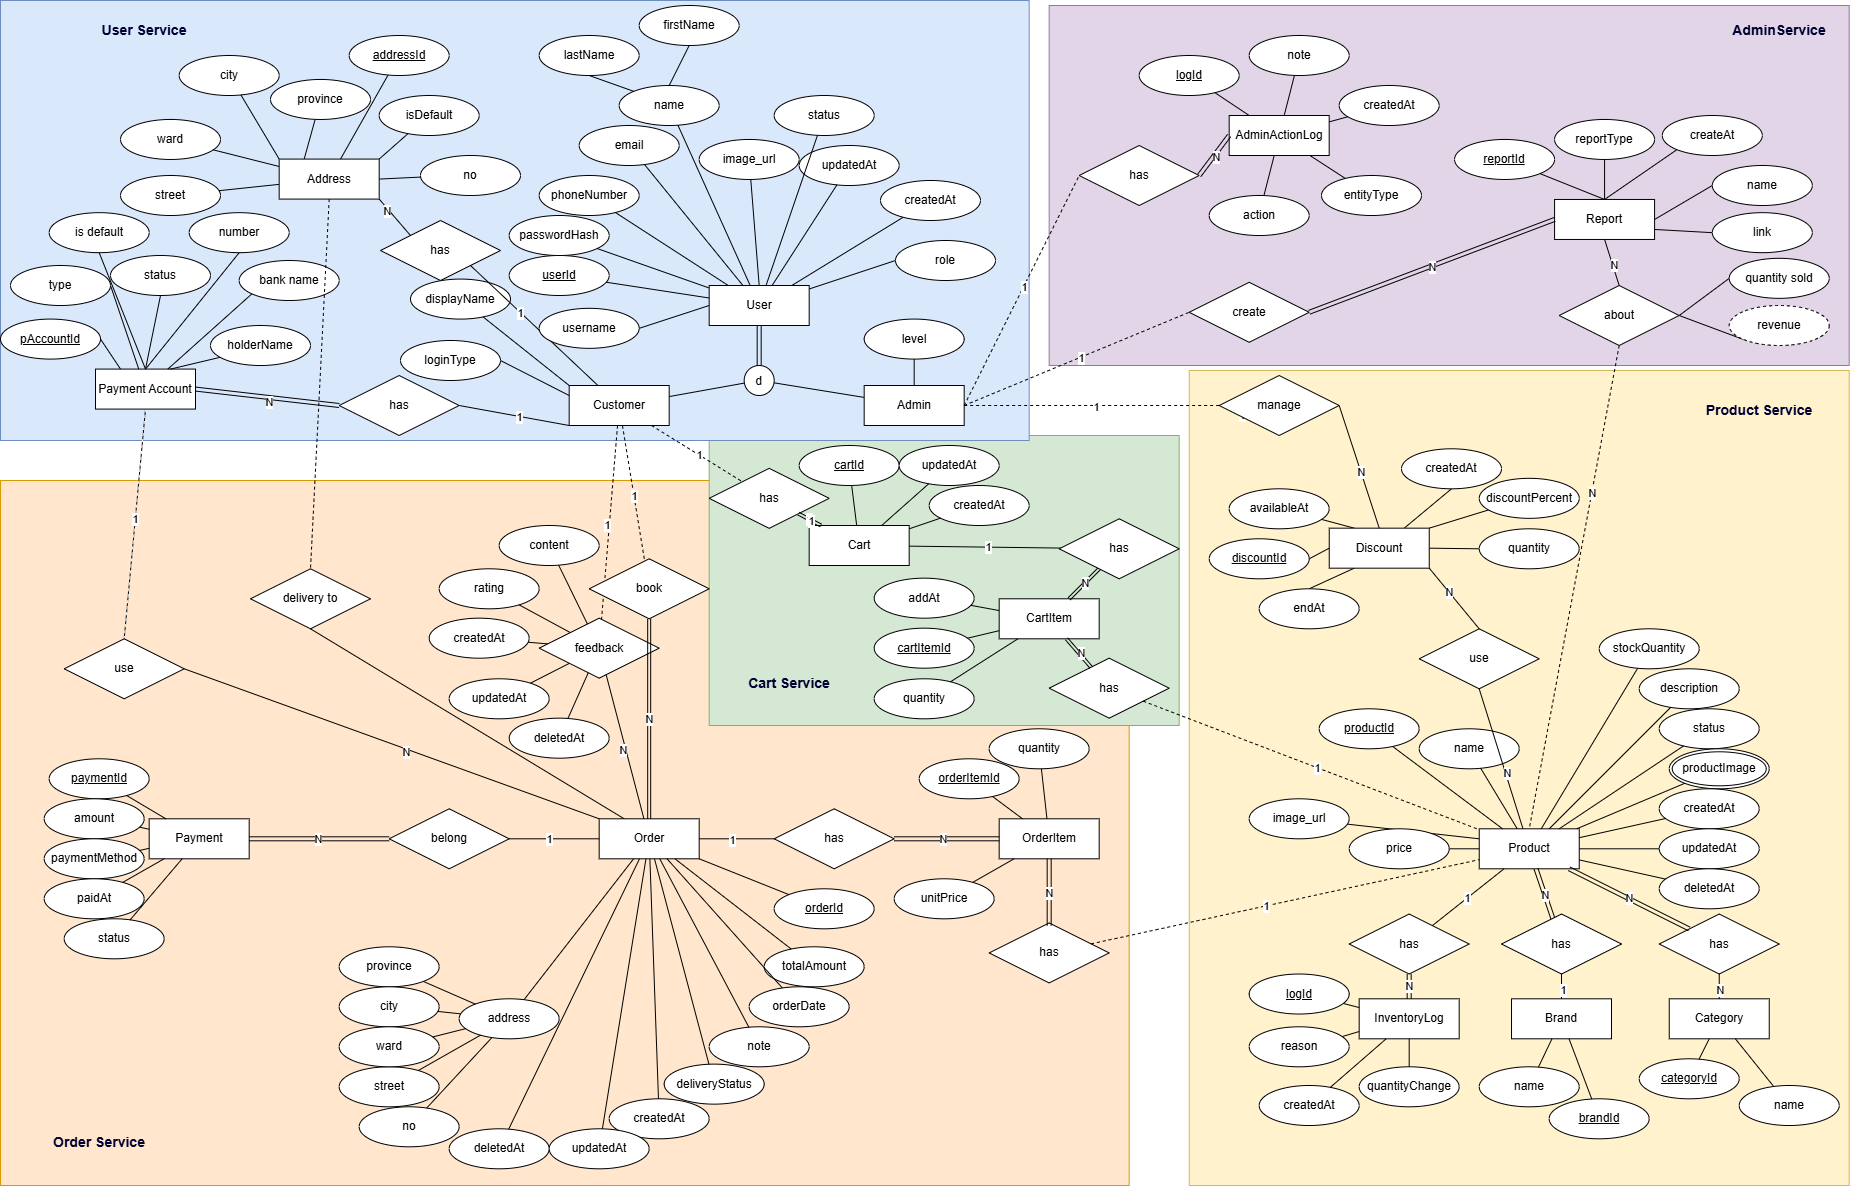
\includegraphics[width=0.9\linewidth]{images/erd/erd.png}
    \vspace{0.5cm}
    \caption{Sơ đồ ERD}
    \label{fig:erd_overview}
\end{figure}

Sơ đồ ERD tổng quan mô tả các thực thể chính của từng domain trong hệ thống. Mỗi nhóm thực thể được tổ chức tách biệt theo chức năng. Các mối quan hệ giữa chúng chỉ mang tính chất tham chiếu logic nhằm mô tả dòng dữ liệu, không phải là ràng buộc vật lý trong cơ sở dữ liệu.

\begin{figure}[H]
    \centering
    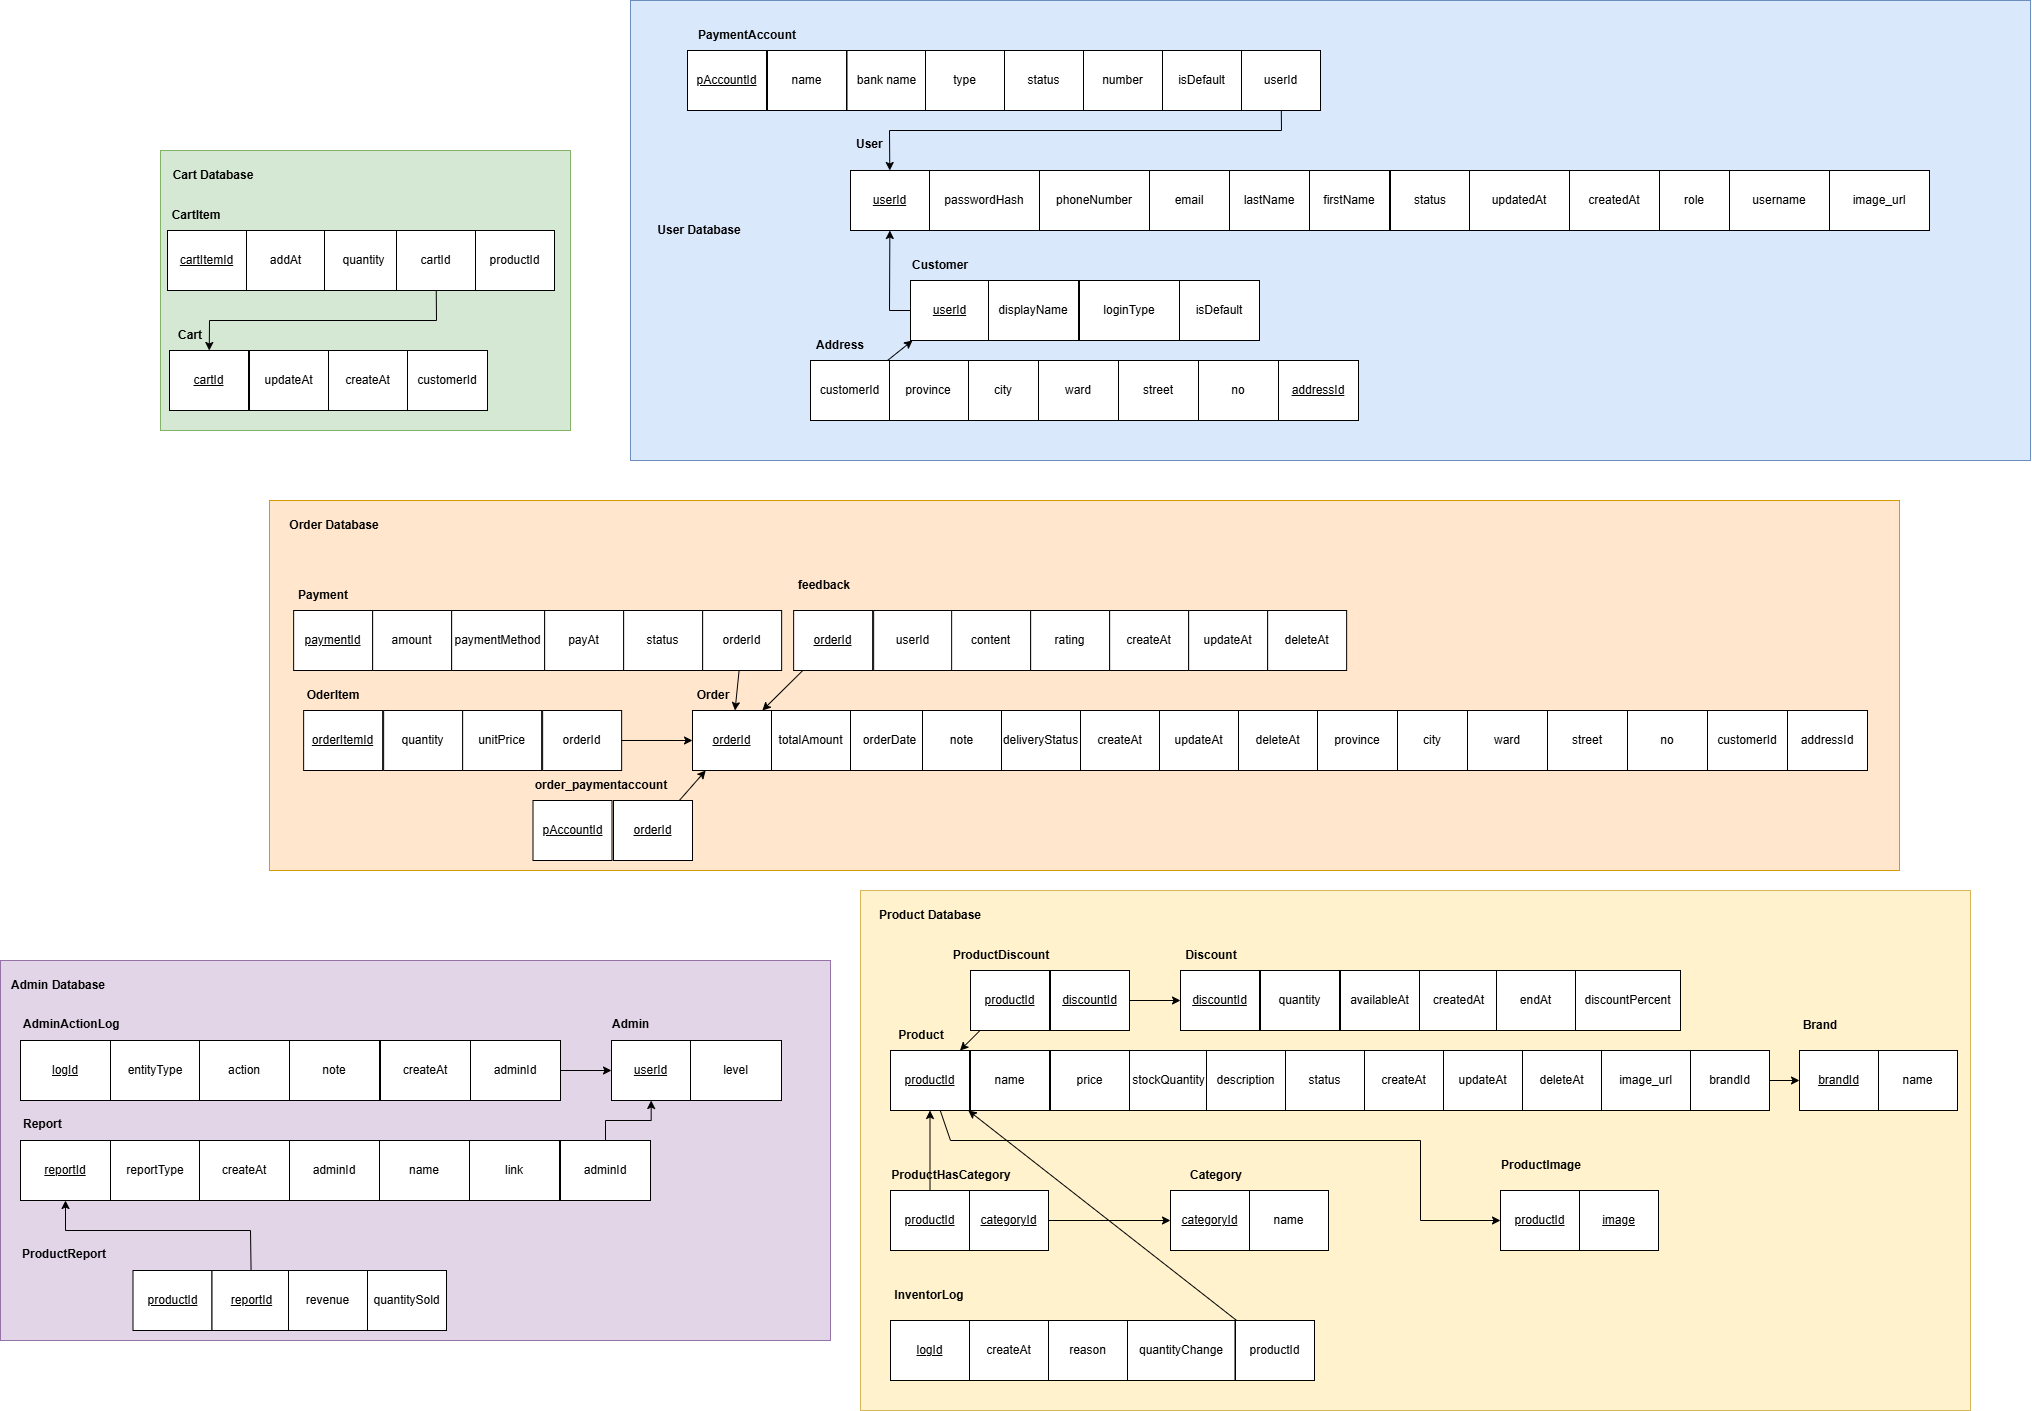
\includegraphics[width=0.9\linewidth]{images/erd/erd_mapping.png}
    \vspace{0.5cm}
    \caption{Sơ đồ ánh xạ ERD}
    \label{fig:erd_mapping}
\end{figure}

Sơ đồ ánh xạ ERD mô tả cách các thực thể được chuyển đổi sang mô hình lưu trữ trong từng microservice. Thay vì sử dụng khóa ngoại, mỗi bảng lưu trữ các định danh cần thiết (ID) để hỗ trợ giao tiếp giữa các dịch vụ hoặc đồng bộ dữ liệu. Cách tiếp cận này giúp hệ thống linh hoạt hơn, dễ mở rộng và phù hợp với các mô hình giao tiếp như event-driven và API orchestration.
